\documentclass{article}
\usepackage{graphicx}
\usepackage{authblk}
\usepackage{amsmath}
\usepackage{listings}

\begin{document}


\title{THEORETICAL NEUROSCIENCE II \\ EXERCISE - OCULAR DOMINANCE}
\date{27 Mai. 2013}
\author[1]{Yunus Emre Demiray, Taygun C. Uzuneser, \c{S}eyma Bayrak\thanks{seyma.bayrak@st.ovgu.de}}
\affil[1]{\footnotesize  Otto von Guericke University of Magdeburg}
\maketitle

\newpage

\section{Input Correlations}
We consider the rates of two LGN afferents, $u_R$ from the right eye and $u_L$ from the left eye such that they are binary, either 1 or 0, and their average is 0.5. The first task is to generate different input pairs of ($u_R,u_L$). The joint probabilities are defined as the following by a limiting $\gamma$ value.

\begin{equation*}
u_{R,L} \;\; \epsilon \;\;\{0,1\} \;\;\;\;\;\;\ \langle u_R \rangle = \langle u_L \rangle = \frac{1}{2}
\end{equation*}
\begin{equation*}
  p_1=p_0=\frac{1}{2} \;\;\;\;\;\;\ p_{11}=p_{00}=\frac{\gamma}{4} \;\;\;\;\;\;\ p_{01}=p_{10}=\frac{1}{2}-\frac{\gamma}{4} \;\;\;\;\;\;\ 0\leq \gamma \leq 2 
\end{equation*}

\begin{itemize}
 \item Use these probabilities to derive the correlation and covariance matrices for chosen values of $\gamma$, both analytically and numerically.
\end{itemize}
\begin{equation*}
 c_S= \langle u_L u_L \rangle - \langle u_L \rangle^2 =\langle u_R u_R \rangle - \langle u_R \rangle^2=\sum_{u_{R,L} \; \epsilon\{0,1\}} p_R .u_R .u_R-(\frac{1}{2})^2 
\end{equation*}
\begin{equation*} 
= p_1u_1u_1 -\frac{1}{4}=\frac{1}{2}.1.1 -\frac{1}{4}=\frac{1}{2}-\frac{1}{4}=\frac{1}{4} \
\end{equation*}

\begin{equation*}
 c_D=\langle u_R u_L \rangle - \langle u_R \rangle . \langle u_L \rangle  =\sum_{u_{R,L} \; \epsilon\{0,1\}} p_{RL}.u_R.u_L-\frac{1}{2}.\frac{1}{2}
\end{equation*}
\begin{equation*}
 =p_{00}.0.0+p_{01}.0.1+p_{11}.1.1+p_{10}.1.0 -\frac{1}{4}=\frac{¸\gamma}{4}-\frac{1}{4}=\frac{1}{4}(\gamma-1)
\end{equation*}
The covariance matrix turns out to be the following:
\begin{equation}
\ C= \left ( \begin{array}{cc} c_S & c_D \\ c_D & c_S \end{array} \right ) \  =  \left ( \begin{array}{cc} \frac{1}{4} & \frac{1}{4}(\gamma-1) \\ \frac{1}{4}(\gamma-1) & \frac{1}{4} \end{array} \right ) \ 
\end{equation}

Now, let us calculate the coefficients for the correlation matrix.
\begin{equation*}
 q_S=\langle u_R^2 \rangle = \langle u_L^2 \rangle=\sum_{u_{R,L} \; \epsilon\{0,1\}} p_R .u_R.u_R=p_0.0.0+p_1.1.1=\frac{1}{2} 
\end{equation*}
\begin{equation*}
 q_D=\langle u_R u_L \rangle=\sum_{u_{R,L} \; \epsilon\{0,1\}} p_{RL} .u_R.u_L=\frac{\gamma}{4} 
\end{equation*}
The correlation matrix turns out to be the following:
\begin{equation}
\ Q= \left ( \begin{array}{cc} q_S & q_D \\ q_D & q_S \end{array} \right ) \  =  \left ( \begin{array}{cc} \frac{1}{2} & \frac{\gamma}{4} \\ \frac{\gamma}{4} & \frac{1}{2} \end{array} \right ) \ 
\end{equation}
The assignment asks for comparing the analytically calculated matrix in equation 1 with the numericlally calculated one. For a better understanding, the comparison is done 5 times with different $\gamma$ values such that $\gamma$=[0 0.25 0.5 0.75 1]. Both analytic and numerical solutions for covariance matrices for different $\gamma$ values are introduced below.

\begin{equation*}
 \gamma=0, \ C_{anly} =  \left ( \begin{array}{cc} 0.2500 & -0.2500 \\ -0.2500 & 0.2500 \end{array} \right ) \  \ C_{num} =  \left ( \begin{array}{cc} 0.2619 & -0.2499 \\ -0.2499 & 0.2619 \end{array} \right ) \
\end{equation*}

\begin{equation*}
 \gamma=0.25, \ C_{anly} =  \left ( \begin{array}{cc} 0.2500 & -0.1875 \\ -0.1875 & 0.2500 \end{array} \right ) \  \ C_{num} =  \left ( \begin{array}{cc} 0.2460 & -0.1910 \\ -0.1910 & 0.2460 \end{array} \right ) \
\end{equation*}

\begin{equation*}
 \gamma=0.5, \ C_{anly} =  \left ( \begin{array}{cc} 0.2500 & -0.1250 \\ -0.1250& 0.2500 \end{array} \right ) \  \ C_{num} =  \left ( \begin{array}{cc} 0.2358 & -0.1335 \\ -0.1335 & 0.2358 \end{array} \right ) \
\end{equation*}

\begin{equation*}
 \gamma=0.75, \ C_{anly} =  \left ( \begin{array}{cc} 0.2500 & -0.0625 \\ -0.0675 & 0.2500 \end{array} \right ) \  \ C_{num} =  \left ( \begin{array}{cc} 0.2510 & -0.0550 \\ -0.0550& 0.2510 \end{array} \right ) \
\end{equation*}

\begin{equation*}
 \gamma=1, \ C_{anly} =  \left ( \begin{array}{cc} 0.2500 & 0 \\ 0 & 0.2500 \end{array} \right ) \  \ C_{num} =  \left ( \begin{array}{cc} 0.2399 & 0 \\ 0 & 0.2399 \end{array} \right ) \
\end{equation*}

The provided MATLAB function \textbf{ShowEigen.m} plots the eigenvectors and eigenvalues for the numerically calculated \textbf{C} matrices for the different $\gamma$ values as the following.

\begin{center}
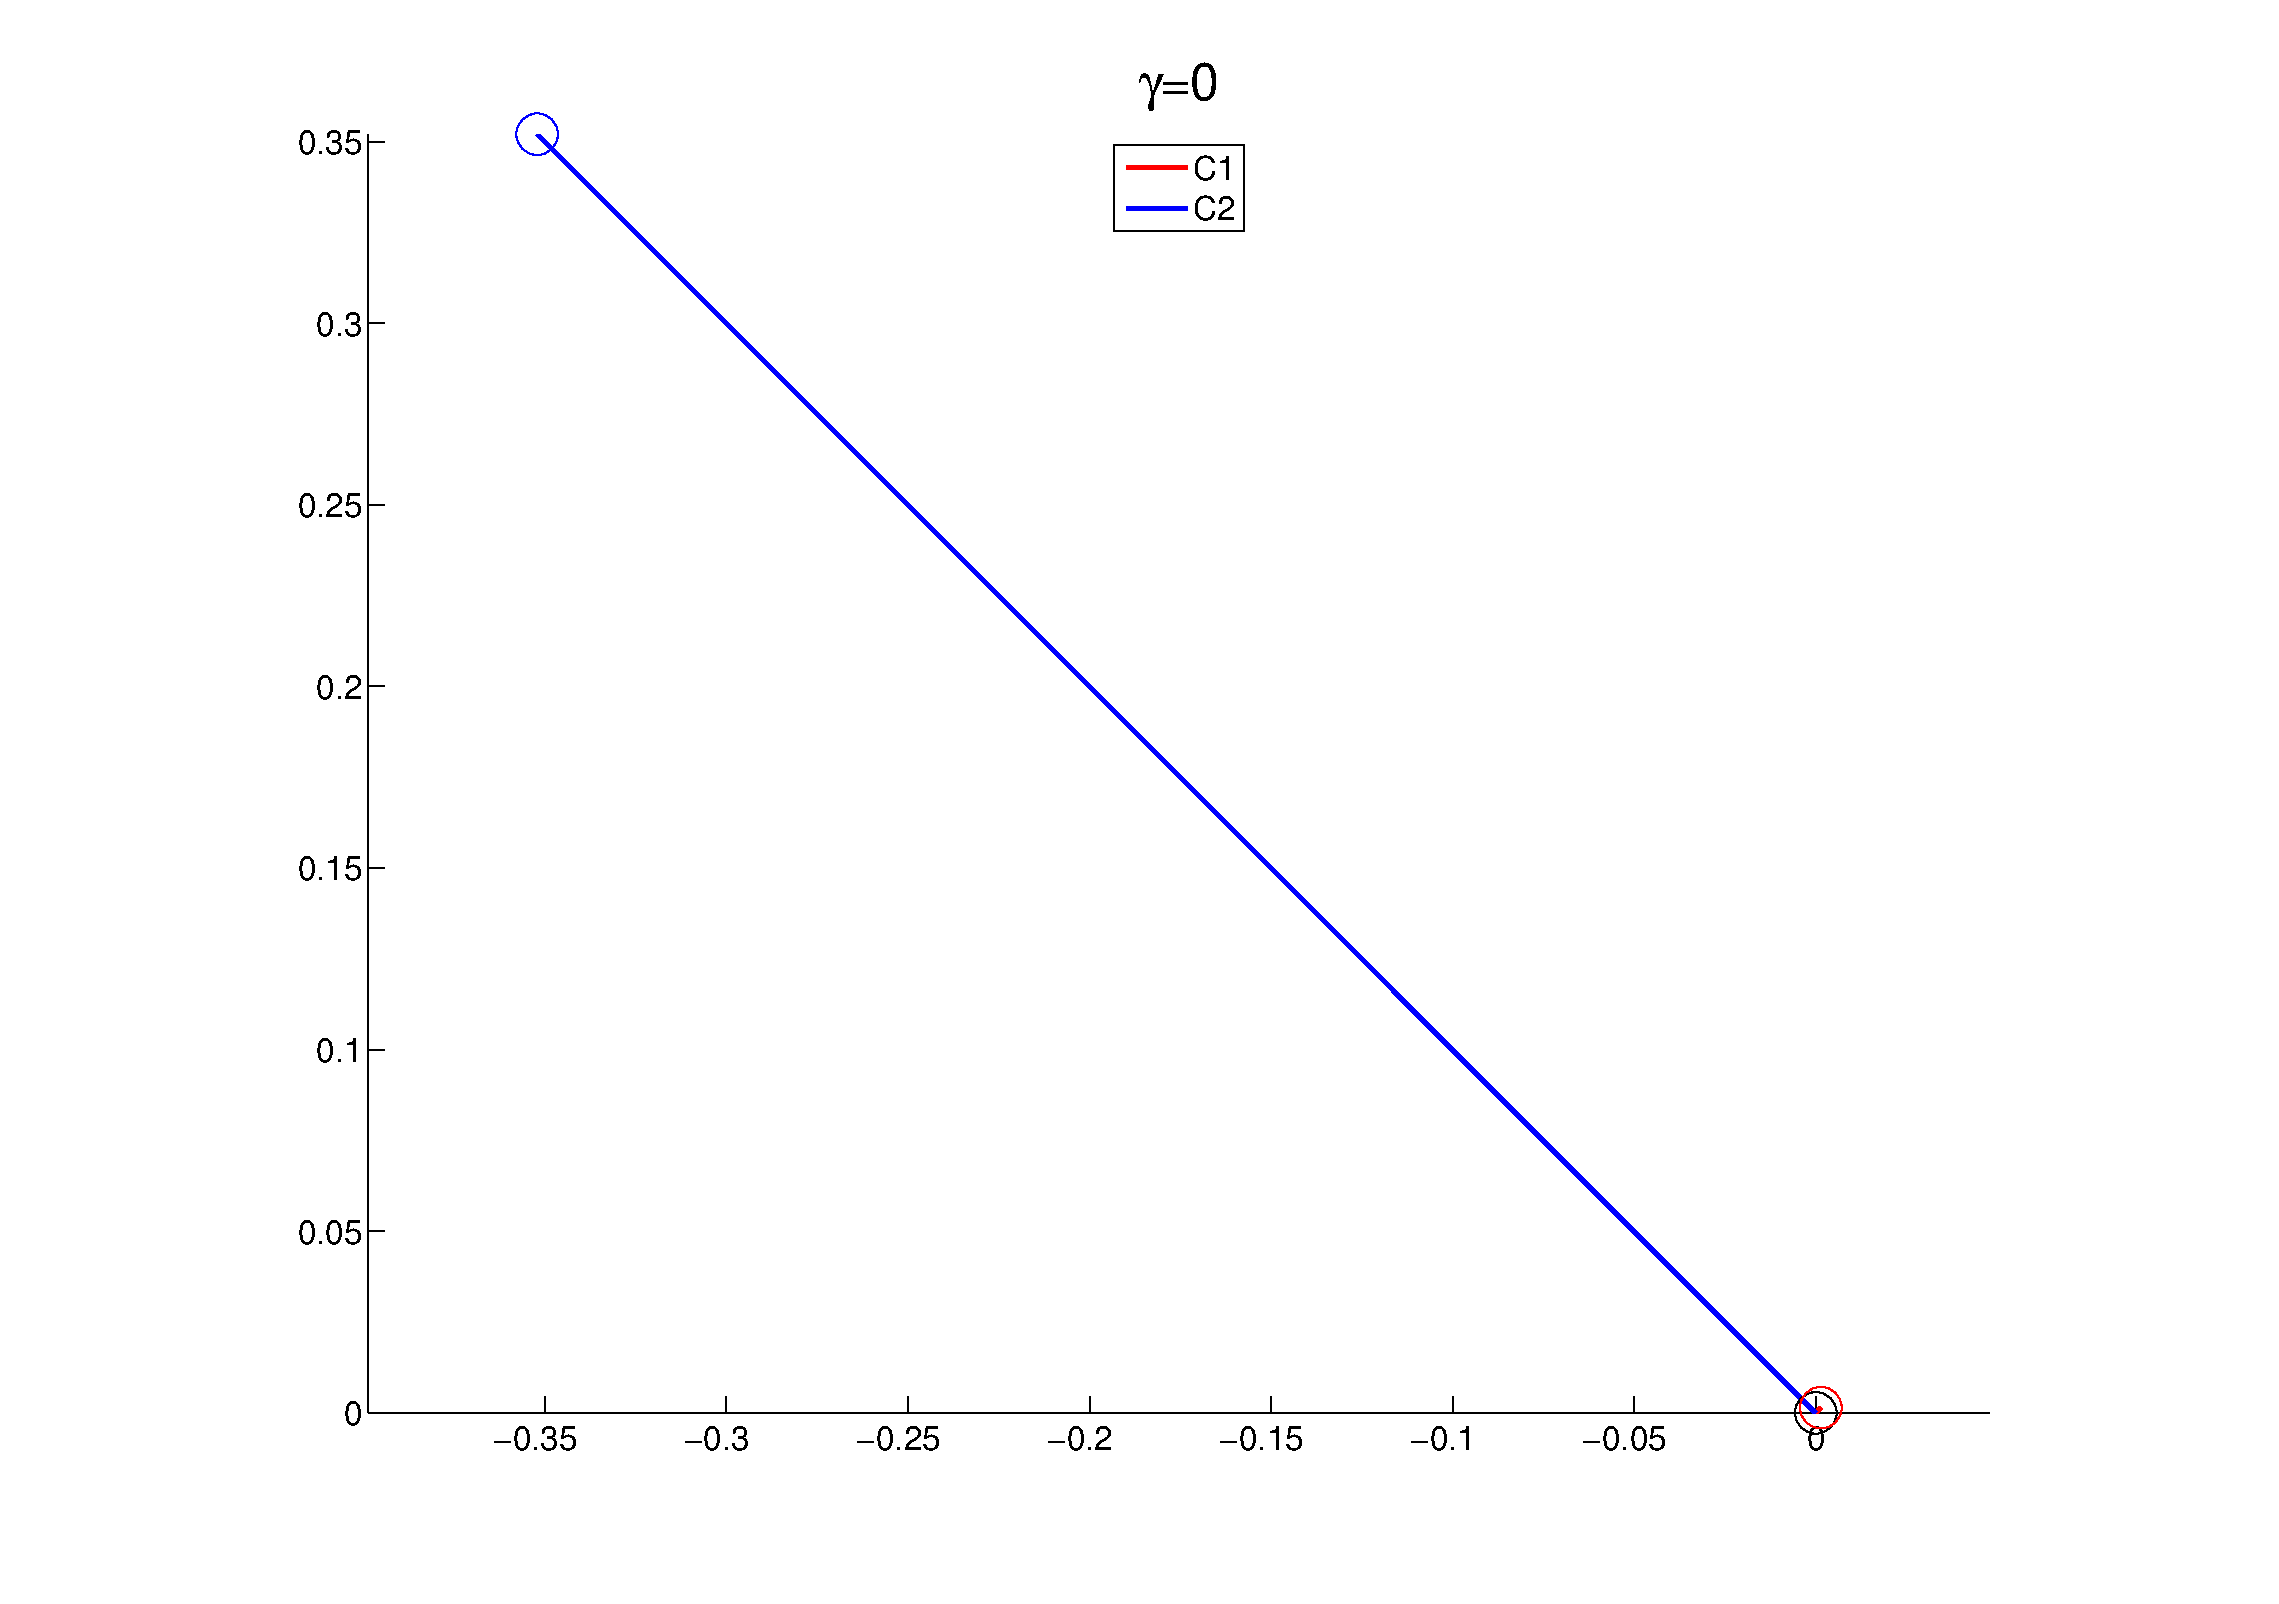
\includegraphics[width=\textwidth]{eigen1.eps}
% tau4_M1.eps: 0x0 pixel, 300dpi, 0.00x0.00 cm, bb= -304   -42   918   834
\begin{footnotesize}
 Figure 1, $\gamma=0$
\end{footnotesize}
\end{center}

\begin{center}
\includegraphics[width=\textwidth]{eigen2.eps}
% tau4_M1.eps: 0x0 pixel, 300dpi, 0.00x0.00 cm, bb= -304   -42   918   834
\begin{footnotesize}
 Figure 2, $\gamma=0.25$
\end{footnotesize}
\end{center}

\begin{center}
\includegraphics[width=\textwidth]{eigen3.eps}
% tau4_M1.eps: 0x0 pixel, 300dpi, 0.00x0.00 cm, bb= -304   -42   918   834
\begin{footnotesize}
 Figure 3, $\gamma=0.5$
\end{footnotesize}
\end{center}

\begin{center}
\includegraphics[width=\textwidth]{eigen4.eps}
% tau4_M1.eps: 0x0 pixel, 300dpi, 0.00x0.00 cm, bb= -304   -42   918   834
\begin{footnotesize}
 Figure 4, $\gamma=0.75$
\end{footnotesize}
\end{center}

\begin{center}
\includegraphics[width=\textwidth]{eigen5.eps}
% tau4_M1.eps: 0x0 pixel, 300dpi, 0.00x0.00 cm, bb= -304   -42   918   834
\begin{footnotesize}
 Figure 5, $\gamma=1$
\end{footnotesize}
\end{center}


\end{document}

